\documentclass[]{UCD_CS_FYP_Report}
\usepackage{graphicx}
\usepackage{listings}
\usepackage{hyperref}
\hypersetup{
    colorlinks=true,
    linkcolor=blue,
    filecolor=magenta,      
    urlcolor=cyan,
}
\lstset{
    mathescape=true,
    basicstyle = \ttfamily
}
%\usepackage[backend=biber,style=chicago-authordate]{biblatex}
\usepackage[backend=biber,style=nature]{biblatex}
\addbibresource{references.bib}


%%%%%%%%%%%%%%%%%%%%%%
%%% Input project details

\def\studentname{Student MacStudent}% Edit with your name
\def\studentid{0600001}% Edit with your student id
\def\projecttitle{Foundations Report} % Edit with you project title
\def\supervisorname{Professor MacProf}


\begin{document}
\maketitle

%%%%%%%%%%%%%%%%%%%%%%
%%% Table of Content

\tableofcontents
%\pdfbookmark[0]{Table of Contents}{toc}\newpage
%\newpage


%%%%%%%%%%%%%%%%%%%%%%
%%% Your Abstract here
\abstract
Provide a short description here (about 150-200 words) of your project. Do not go into fine detail, but offer a strategic overview of the project’s aims. An abstract should whet the appetite for what comes next, not quench it with details.


%%%%%%%%
\chapter{Project Specification}
Repeat here the main demands of the project as provided in the original project specification. Do not repeat the general introduction, just the Core and Advanced goals against which your progress will be judged.


%%%%%%%%
\chapter{Introduction}
Introduce your vision of the project here. Describe the domain of the project, and the intended application. A well-written report will answer three key questions: What am I doing in this project? Why is it worth doing? How do I plan to go about it? In this introductory section, offer a concise answer to the What, and follow-up with a compelling account of the Why. Leave the How to a subsequent section. Do not try to do too much in any single section of the report. By providing details in a logical order, you will show that you have a plan for the report and the project.

%%%%%%%%
\chapter{Related Work and Ideas}
A key task of this first report is to establish a baseline against which your later work will be judged. Your FYP project does not exist in a vacuum, and its central problem, or a variant thereof, will have been tackled by others before you. In this section, you should describe how previous approaches have tackled the problem, and clearly articulate the state of the art (or SOA) for your project.

For research-oriented projects, this task will be time-consuming but relatively straightforward. You should read past works on the subject, summarise the main points, pros and cons, and root out the previous works that they cite in turn. You may use Wikipedia as a secondary source only, which is to say that it can be a useful first port of call on many topics but not a source that should be liberally cited. Rather, use Wikipedia as a hub for gathering references to primary work in the field (original papers and reports), then read and summarise those. Do not quote a work that you have not read, unless you are quoting someone else’s view of that work. Never use another writer’s words as your own. Place any extracts from another’s work in double quotes, and attribute the quotation to its author with a citation. It is a very low act to plagiarise another’s work and take credit for their words, so tread carefully. Even unintentional plagiarism is still plagiarism.

For more application-oriented projects, you are still expected to survey other solutions, either for the given problem or for similar problems, and also consider applications that share functionality or design principles with your own. In short, this section is the core of your report regardless of what kind of project you do.

%%%%%%%%
\chapter{Data Considerations}
In this section you should characterise the nature and scale of the data you are working with. Outline the shape of the data, where you expect to obtain it, and the size of the data. Is it static or dynamic, local or remote, stored or streaming? Is it raw or structured? Is it unfiltered user data, or is it curated by a specialist? What is your rationale for using this data and not other data? If your project looks at callout times for Spanish ambulances, usage rates of French parking lots, alcohol consumption in Germany, and so on, then explain why you are not using Irish data for the project. Indicate the data-cleaning processes that you anticipate will be necessary. What licensing restrictions, if any, apply to your data? Will you be making this data public after your project is completed? Are there any privacy or ethical issues with how the data is to be collected or used? If so, discuss here.

Some or many of these questions may be moot in the case of specific projects, but you should provide compelling answers to any that seem relevant. Since this provides the foundation for your project, your reviewers will be looking closely.

%%%%%%%%
\chapter{Outline of Approach}
In this section present an outline of your considered approach to the problem at the centre of your project. Clearly present your design choices, or your choice of algorithms, and any pertinent model parameters. For instance, if you plan to use a genetic algorithm, outline here a sense of your fitness function, major variables, population size, and so on, so that your reviewers can critique your choices. If you opt for a neural architecture, describe your chosen framework, and motivate the number and kinds of layers in your network. In short, be specific about the choices you are committing to at this stage. Being vague and non-specific will not help your case, as your report will be graded in large part on the specificity and perceived wisdom of your choices. Remember also that feedback is intended to help you as you progress to the next stage of your project. If you give reviewers little to chew on, they will not be able to give you specific feedback and guidance.


%%%%%%%%
\chapter{Project Workplan}
In this section you will present a work plan for the remainder of your project. Show that you have considered the issues carefully, and that you can be trusted to lead a research or development effort. Be as specific as you can about the time you expect to allocate to each work component, and the dependencies they have to each other. A Gantt chart is helpful in this respect, but do show some sense in how you present your plan. A naïve understanding makes for a simplistic plan.

A key part of a successful project is evaluation. It is not enough to just state that your project is a success, or that your friends seem to like it. You must have a plan for evaluating the end result. How you evaluate will depend on the nature of your project, and you should have a serious conversation with your supervisor about evaluation before you get to this stage. Will your work yield quantitative results that can be compared to past work or to established benchmarks? Does your work consider different configurations of a system or a solution that you can compare to each other, allowing you to empirically find the best one? Do you have a sample user pool for your planned application, and are they willing to give you structured qualitative and quantitative feedback (e.g. via a questionnaire)? However you plan to evaluate your project, please sketch your intentions here.

%%%%%%%%
\chapter{Summary and Conclusions}
In this section you will sum up your report, draw some conclusions about your work so far, and make some general observations about the work to come. You may also use this opportunity to express points of view, or make factual claims, that are more pertinent here than in other sections of the report. If your project raises some ethical concerns, for example about how data or users are treated, then address them here in a thoughtful manner.

Regarding this document, here are some concluding points that you should keep in mind when writing your own. You may use screenshots in your report, but do not overfill your report with them, or with figures of any kind. Make sure that figures earn their keep, and are not just present as space fillers or as eye candy. If you use diagrams or figures from other people’s work, including the web, be sure to cite the creator in the corresponding caption. All things being equal, it is better to construct your own figures than to copy and paste those of others. In any case, always make sure that your images are readable, do not suffer from pixelation or aliasing effects, and that each is clearly numbered, captioned and meaningfully referenced in the main body of the text.

Ensure that there is a cohesive argument expressed in the text of the report and that it is not simply a bag of diagrams, screenshots and wishful thinking. Every report should tell a story, so know what story you want to tell. When you include images, make sure they are readable and truly add to the discussion.

Make sure your language is professional throughout, and steer a course between pompous and colloquial. Maintain authorial distance and do not overuse “me,” “I” and “our.” Your are writing for a professional audience who will judge you on the quality of your prose, so use a grammar and a spelling checker.

Use LaTeX if you wish – this is recommended if you plan to use mathematical formulae in your report, but in any case, keep the general spacing and font/style you find here (Single or 1.5 spacing, 12 pt. font for text, etc.). Be sure to submit a PDF (never a .DOC or .DOCX file) as your report. If you prepare your report in MS Word, as this document has been, save it as a PDF before you submit it. Overall it should be about 18 – 20 pages, including figures, front matter and references, A significant portion of the report will be textual, with approx.. five or six thousand words. Do not rely on images or other filler to write your report for you.
The dates and means of submission will be communicated to you separately.


%%%%%%%%%%%%%%%%%%%%%%
%%%% Latex help.
\chapter{Latex Pointers}

TODO remove.

This chapter contains some examples on the usage of latex. Do not include in your final report.

\section{Figures}
From time to time, it's necessary to add pictures to your documents. Using LaTeX all pictures will be indexed automatically and tagged with successive numbers when using the figure environment and the graphicx package. We can reference the figure below using its label like this: Fig. \ref{fig:test_plot}.
\begin{figure}[H]
  \centering
  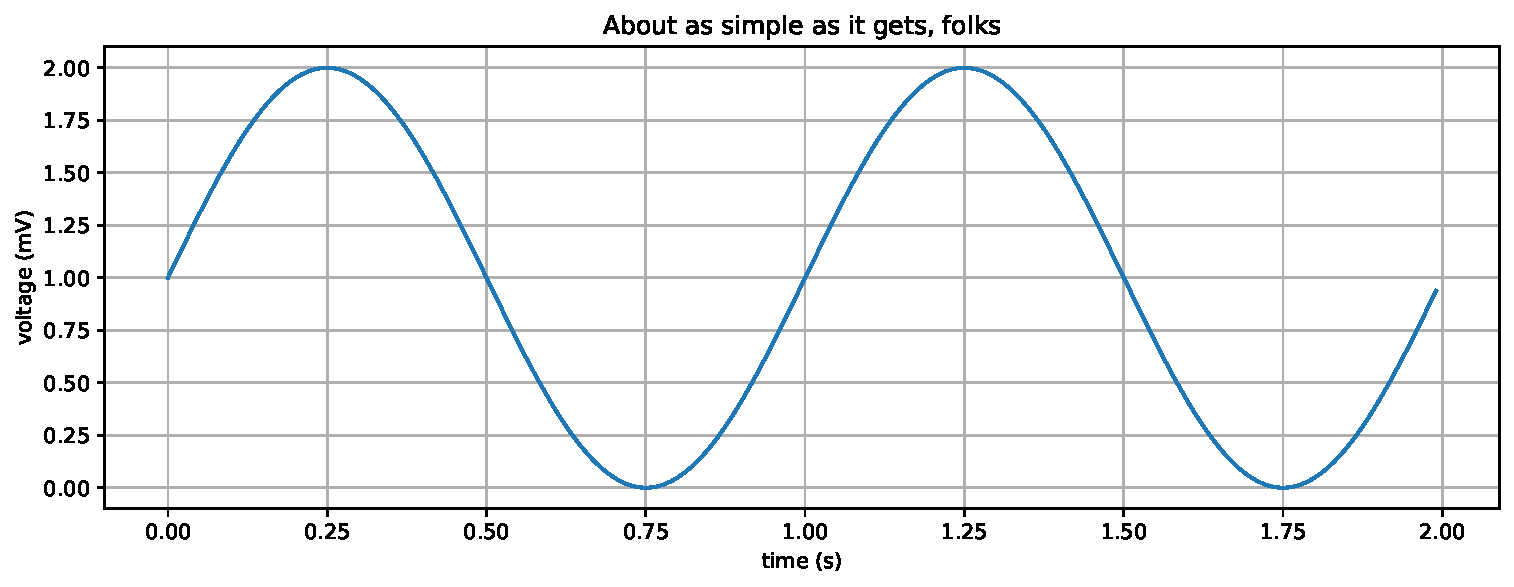
\includegraphics[width=0.8\linewidth]{./assets/images/test-plot.pdf}
  \caption{A sample graph}
  \label{fig:test_plot}
\end{figure}

Lots more information in this \href{https://www.latex-tutorial.com/tutorials/figures/}{tutorial}.


\section{Code Listing}
You can list code using the \emph{listings} package:

\begin{lstlisting}[language=Python,caption=Borg Pattern]
class Borg(object):
    __shared_state = {}

    def __init__(self):
        self.__dict__ = self.__shared_state
        self.state = 'Init'

    def __str__(self):
        return self.state
\end{lstlisting}

Lots more examples \href{https://www.overleaf.com/learn/latex/Code_listing}{here}.

\section{Math}
Here \ref{eq:limit} is an example of including an equation
\begin{equation}
  \lim_{x\to\infty} f(x)
  \label{eq:limit}
\end{equation}

More examples \href{https://www.latex-tutorial.com/tutorials/amsmath/}{here} and \href{https://www.overleaf.com/learn/latex/Mathematical_expressions}{here}.



\section{References}
Look up the bibtex references on google scholar or import from Mendeley or other reference managers. Add the bibtex snippet to the \emph{references.bib} file. Then cite the reference like this:

As explained in \cite{knuth2014art}, we also find that...

Lots more details \href{https://www.latex-tutorial.com/tutorials/bibtex/}{here}.



%%%%%%%%%%%%%%%%%%%%%%
%%% Acknowledgements
\chapter*{Acknowledgements}
In your Acknowledgements section, give credit to all the people who helped you in your project.


%%%% ADD YOUR BIBLIOGRAPHY HERE
\printbibliography

%%%%
%%%% maybe code listing here?

%%%%
\end{document}
%\end{article}
